\begin{problem}
  Let $\displaystyle f(x) = \frac{1 + x}{1 + x^3}$.
  \begin{enumroman}
    \item Find a largest subset $U \subseteq \R$ where $f$ is well-defined.
      Is $f$ continuous on $U$?~\label{problem:1a}
      
      \begin{answer}
        Since $f$ is a rational function where the numerator and
        denominator consist of polynomial functions,
        it is well-defined where the denominator is nonzero.
        Thus, $U = \R \setminus \{-1\}$.

        % To show that $f$ is continuous on $U$, we show that
        % $f$ is continuous at every point in $U$.
        \step
        Since $U$ is open and $f$ is a rational function, $f$ is continuous
        on $U$ (\crim{
          We proved this result in class.
        }).
      \end{answer}

    \newpage
    \item Let $U$ be as in part~\ref{problem:1a}.
      Let $g$ be a function such that $g(x) = f(x)$ if $x \in U$. \\
      Is there a way to define $g$ on $\R \setminus U$ to obtain
      a continuous function $g$ on $\R$?~\label{problem:1b}

      \begin{answer}
        \begin{figure}[H]
          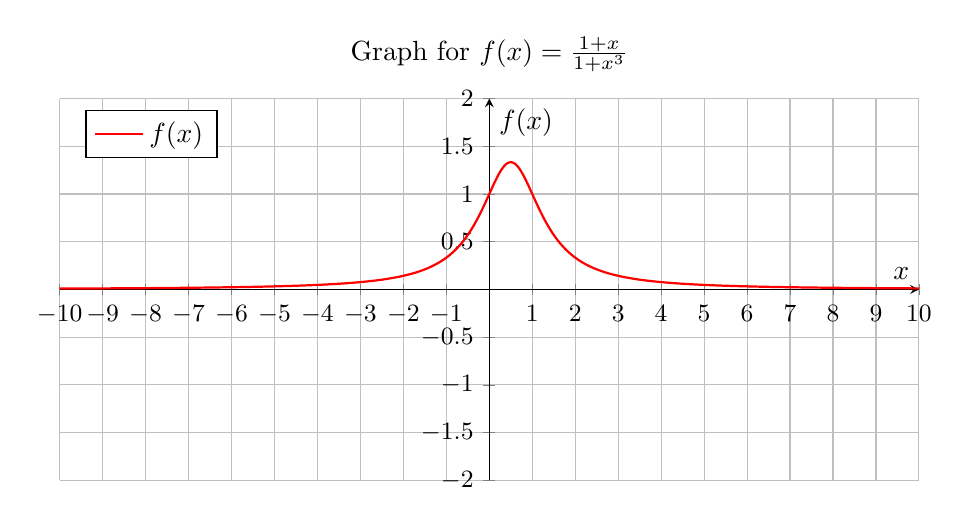
\begin{tikzpicture}
            \begin{axis}[
              title={Graph for $f(x) = \frac{1 + x}{1 + x^3}$},
              xlabel={$x$},
              ylabel={$f(x)$},
              xmin=-10, xmax=10,
              ymin=-2, ymax=2,
              axis lines=center,
              grid=major,
              xtick={-10,-9,...,10},
              ytick={-2,-1.5,...,2},
              tick label style={font=\small},
              legend pos=north west,
              scale only axis,
              width=0.9\textwidth,
              height=0.4\textwidth
            ]
          \addplot[red, thick, samples=400, domain=-10:10] {(1+x)/(1+x^3)};
          \legend{$f(x)$}
          \end{axis}
          \end{tikzpicture}
          \caption*{Note: value at $x = -1$ is not defined, which is not demonstrated in this plot.}
        \end{figure}

        For $g$ to be continuous on $\R$, we need to define $g$
        at $-1$ such that $\displaystyle \lim_{x \to -1} g(x) = g(-1)$.
        Since $g$ has an indeterminate form at $-1$, 
        we use L'H\^{o}pital's rule to find the limit:

        \begin{align*}
          \lim_{x \to -1} \frac{1 + x}{1 + x^3}
          &= \lim_{x \to -1} \brackets{\frac{\d}{\d x} (1 + x) \Big/ \frac{\d}{\d x} (1 + x^3)} \\
          &= \lim_{x \to -1} \frac{1}{3x^2} \\
          &= \frac{1}{3}
        \end{align*}

        \step
        Thus, we can define
        \[
          g(x) = \begin{cases}
            f(x) &\text{ if } x \in \R \setminus \set{-1} \\
            \frac{1}{3} &\text{ if } x = -1
          \end{cases}
        \]
        to obtain a continuous function on $\R$.
      \end{answer}
  \end{enumroman}
\end{problem}
